\documentclass[listof=nochaptergap]{report}

\usepackage[utf8]{inputenc}
\usepackage[english]{babel}
\usepackage{geometry}
\usepackage{graphicx}
\usepackage{hyperref}
\usepackage{tikz}
\usepackage{pgfplots}
\usepackage{listings}
\usepackage{minted}
\usepackage{caption}
\usepackage{setspace}

\geometry{
    paper=a4paper,
    top=32mm,
    bottom=32mm,
    left=25mm,
    right=25mm
}

\setminted[cpp]{
    frame=lines,
    framesep=2mm,
    fontsize=\footnotesize,
    linenos,
    breaklines
}

\renewcommand{\lstlistingname}{Algorithm}% Listing -> Algorithm
\renewcommand{\lstlistlistingname}{List of \lstlistingname s}% List of Listings -> List of Algorithms



\begin{document}
    \begin{titlepage}
        \noindent
        \includegraphics[width=1.0\textwidth]{images/Q04_HTW_Berlin_Logo_quer_pos_FARBIG_RGB.jpg}


        \vspace{2cm}

        \begin{center}
            \noindent
            \huge{\textbf{Grayscale, RGB to HSV and Emboss parallelized with OpenMP}}

            \vspace{1cm}

            \noindent
            \LARGE{Module: Programmierkonzepte und Algorithmen}

            \vspace{1cm}

            \noindent
            \small{\today}
        \end{center}

        \vfill

        \noindent
        \begin{minipage}[t]{0.5\textwidth}
            \begin{flushleft}
                \textbf{Student}\\
                Name: Christoph Stach\\
                Matrikel-Nr: 0555912                
            \end{flushleft}
        \end{minipage}
        \begin{minipage}[t]{0.5\textwidth}
            \begin{flushright}
                \textbf{Dozent}\\
                Mykyta Kovalenko\\
            \end{flushright}
        \end{minipage}
    \end{titlepage}

    \tableofcontents

    \chapter{Introduction}

\noindent
This document includes the technical documentation about various task implemented with OpenMP. The goal of this document is to show the outcomes of various algorithms and compare their performance with the OpenCV library. OpenMP is a library that enables easy to use parallel computing on multiple CPUs. To demonstrate its capabilities the author implemented a Grayscale-, a RGB2HSV- and an Emboss-Algorithm. All of them consist of two For-Loops, which loop over all pixels of an image.\\

\noindent
The run time of each algorithm was measured with different usage scenarios of OpenMP. To parallelize a program into multiple threads, OpenMP offers the \mintinline{cpp}{#pragma omp parallel for} compiler directive for For-Loops.  The author used OpenMP on the outer For-Loop, the inner For-Loop and both For-Loops. The results are shown in the following performance test diagrams for each algorithm. Also the results, the algorithms produce, are demonstrated and the implementation is given accordingly.\\

\noindent
All performance tests were done on a Dell XPS 15 9955, with a Intel Core i7, 16GB ram and a nVidia GeForce GTX 960m. Each test was run 200 times and the arithmetic mean was of all iterations was taken. \\

\noindent
The source code, this document is based on, is hosted on \url{http://github.com} under the URL \url{http://github.com/christophstach/openmp-emboss}.


    \chapter{Implementation}

\section{Project setup}

To make the project runnable on different machines the CMake\footnote{\url{https://cmake.org/}} was chosen as a build tool. Under Linux uses gcc and g++ to compile C and C++ projects. The project uses OpenCV to load images and compare results. All images are converted to 4-channel images. This was necesary to make the handwritten algorithms compatible with all kinds of images. To further improve performance it would be beneficial to let the algorithms handle different types of image data themself in the future.\\

The configuration for the project can be found in the CMakeList.txt. Also the package manager CPM\footnote{\url{https://github.com/TheLartians/CPM.cmake}} is used. CPM extends CMake to easily download third party libraries from git hosting services.\\

The library cxxopts\footnote{\url{https://github.com/jarro2783/cxxopts}} was used to add a proper CLI interface and complete concept of the application.

\section{Implementation variants}

Each algorithms is implemented three times to test different implementation strategies. The two for-loops, which loop over each pixel of in image, are implemtend in the following three variants:

\begin{listing}
\begin{minted}{cpp}
#pragma omp parallel for default(none) shared(srcImage, destImage)
for (int row = 0; row < srcImage.rows; row++) {
    for (int col = 0; col < srcImage.cols; col++) {
\end{minted}
\captionof{lstlisting}{For-Loop parallelization variant 1}
\label{listing:forloop1}
\end{listing}



The first one parallelizes the outer for loop. It splits up the amount of rows into equal parts. Then $ n $ threads are created and each thread computes an equal amount of parts. 

\pagebreak

\begin{listing}[H]
\begin{minted}{cpp}
for (int row = 0; row < srcImage.rows; row++) {
    #pragma omp parallel for default(none) shared(srcImage, destImage, row)
    for (int col = 0; col < srcImage.cols; col++) {
\end{minted}
\captionof{lstlisting}{For-Loop parallelization variant 2}
\label{listing:forloop2}
\end{listing}


The second solution creates $ n $ threads and splits each row into small parts of pixels. The rows are computed sequentially and then the columns are computed in parallel.

\begin{listing}[H]
\begin{minted}{cpp}
#pragma omp parallel for collapse(2) default(none) shared(srcImage, destImage)
for (int row = 0; row < srcImage.rows; row++) {
    for (int col = 0; col < srcImage.cols; col++) {
\end{minted}
\captionof{lstlisting}{For-Loop parallelization variant 3}
\label{listing:forloop3}
\end{listing}


The \mintinline{cpp}{# collapse(2)} keyword increases the ttal number of iterations that will be partitioned across the available number of OMP threads\footnote{\url{https://software.intel.com/en-us/articles/openmp-loop-collapse-directive}}.

\section{Grayscale}


To convert an image to grayscale the three color channels needs to be converted to one channel. The remaining channel needs to capture a kind of mean of the other channels. This can be done with different formulars. It is possible to use luminosity formular $ 0.21r + 0.72g + 0.07b $. But this project uses the same formular like OpenCV uses, $ 0.299r + 0.587g + 0.114b $, to make results better comparable. Each pixel of an image is converted by this formular to convert the whole image to a grayscale image.

\section{HSV}

HSV (Hue, Saturation, Value) is a different representation of the RGB (Red, Green, Blue) color-model. It is used to make easy adjustments according to it's components. Usually image programs and \LaTeX \space interpret images as RGB images. This is the reason for the colorful representation of the images.

First all pixel values are devided by $ 255.0 $. For each pixel the maximum and minimum of the color channels is taken and saved into the variables \mintinline{cpp}{cMax} and \mintinline{cpp}{cMin}. Then highest difference is taken as a reference value. The following formular calculates the Hue:

\begin{listing}[H]
\begin{minted}{cpp}
if (cMax == cMin) {
    h = 0;
} else if (cMax == r) {
    h = int(60 * ((g - b) / diff) + 360) % 360;
} else if (cMax == g) {
    h = int(60 * ((b - r) / diff) + 120) % 360;
} else {
    h = int(60 * ((r - g) / diff) + 240) % 360;
}
\end{minted}
\captionof{lstlisting}{HSV algorithm}
\label{listing:hsv1}
\end{listing}


The Saturation is then simply calculated by exucuting \mintinline{cpp}{s = cMax == 0 ? 0 : (diff / cMax);}. The value is just the  \mintinline{cpp}{cMax} variable.

\section{Emboss}

The Emboss algorithm compares every channel each pixel with it's upper left neighbour. The maximum difference is taken as a reference value.


\begin{listing}[H]
\begin{minted}{cpp}
int diffR, diffG, diffB, diff, gray;
auto srcPixel = srcImage.at<cv::Vec4b>(row, col);
auto upperLeftPixel = srcImage.at<cv::Vec4b>(row - 1, col - 1);

diffR = std::abs(srcPixel[2] - upperLeftPixel[2]);
diffG = std::abs(srcPixel[1] - upperLeftPixel[1]);
diffB = std::abs(srcPixel[0] - upperLeftPixel[0]);

diff = std::max(diffR, std::max(diffG, diffB));
\end{minted}
\captionof{lstlisting}{Emboss algorithm 1}
\label{listing:emboss1}
\end{listing}

Afterwards a new gray color is calculated and set for all channels of the destination image. The alpha channel is taken as is from the source image.

\begin{listing}[H]
\begin{minted}{cpp}
gray = 128 + diff;
gray = gray > 255 ? 255 : gray;
gray = gray < 0 ? 0 : gray;

cv::Vec4b destPixel = cv::Vec4b(
    uchar(gray),
    uchar(gray),
    uchar(gray),
    srcPixel[3]
);

destImage.at<cv::Vec4b>(row, col) = destPixel;
\end{minted}
\captionof{lstlisting}{Emboss algorithm 2}
\label{listing:emboss2}
\end{listing}
    % \chapter{HSV}

\section{Performance Tests}

\begin{center}
    \begin{figure}[H]
        \centering

        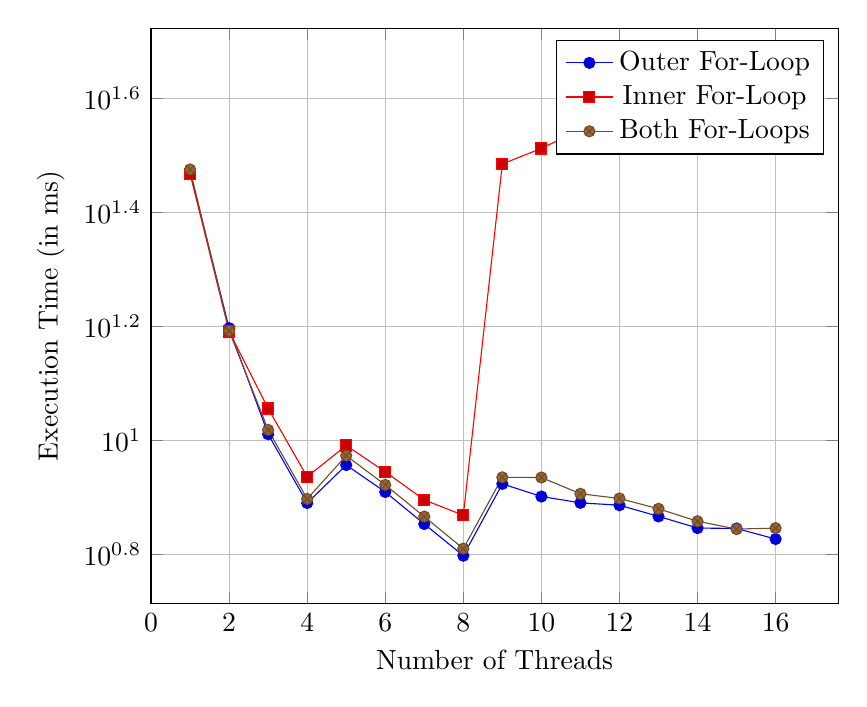
\begin{tikzpicture}
            \begin{axis}[
                title={},
                width=0.85\textwidth,
                xlabel={Number of Threads},
                ylabel={Execution Time (in ms)},
                xmin=0,
                ymin=0,
                ymode=log,
                grid=major
            ]
                \addplot coordinates {
                    (1,29.5366)(2,15.7231)(3,10.2453)(4,7.7598)(5,9.04545)(6,8.11285)(7,7.1297)(8,6.27195)(9,8.3824)(10,7.96645)(11,7.7646)(12,7.69085)(13,7.35195)(14,7.01335)(15,7.00095)(16,6.70895)
                };
                \addlegendentry{Outer For-Loop}

                \addplot coordinates {
                    (1,29.3423)(2,15.5132)(3,11.3651)(4,8.62715)(5,9.78995)(6,8.8026)(7,7.857)(8,7.38445)(9,30.5217)(10,32.4977)(11,35.0829)(12,36.9657)(13,37.1315)(14,39.4836)(15,39.4552)(16,43.51)
                };
                \addlegendentry{Inner For-Loop}
                
                \addplot coordinates {
                    (1,29.8459)(2,15.5525)(3,10.4249)(4,7.89)(5,9.39475)(6,8.3478)(7,7.3445)(8,6.45355)(9,8.6068)(10,8.60125)(11,8.05395)(12,7.9041)(13,7.581)(14,7.2079)(15,6.9847)(16,7.01045)
                };
                \addlegendentry{Both For-Loops}   
            \end{axis}
        \end{tikzpicture}
        \caption{RGB to HSV Performance Tests}
    \end{figure}
\end{center}

\section{Results}

\begin{figure}[H]
    \centering

    \includegraphics[width=0.25\textwidth]{images/dice.png}
    \includegraphics[width=0.25\textwidth]{images/cv-hsv.png}
    \includegraphics[width=0.25\textwidth]{images/own-hsv.png}
    
    \caption{RGB to HSV results of OpenCV (middle) and self-implemented  Algorithm (right)}
    \label{fig:hsv}
\end{figure}

\section{Implementation}

\begin{listing}[H]
    \begin{minted}{cpp}
cv::Mat applyHsvOuter(cv::Mat srcImage, int numThreads = omp_get_num_procs()) {
    cv::Mat destImage(srcImage.rows, srcImage.cols, CV_8UC3);
    omp_set_num_threads(numThreads);

    #pragma omp parallel for default(none) shared(srcImage, destImage)
    for (int row = 0; row < srcImage.rows; row++) {
        for (int col = 0; col < srcImage.cols; col++) {
            auto srcPixel = srcImage.at<cv::Vec3b>(row, col);

            double r = srcPixel[2] / 255.0;
            double g = srcPixel[1] / 255.0;
            double b = srcPixel[0] / 255.0;

            double h, s, v;

            double cMax = std::max(std::max(r, g), b);
            double cMin = std::min(std::min(r, g), b);
            double diff = cMax - cMin;

            if (cMax == cMin) {
                h = 0;
            } else if (cMax == r) {
                h = int(60 * ((g - b) / diff) + 360) % 360;
            } else if (cMax == g) {
                h = int(60 * ((b - r) / diff) + 120) % 360;
            } else {
                h = int(60 * ((r - g) / diff) + 240) % 360;
            }

            s = cMax == 0 ? 0 : (diff / cMax);
            v = cMax;

            cv::Vec3b destPixel = cv::Vec3b(
                    uchar(h / 360.0 * 180.0),
                    uchar(s * 255.0),
                    uchar(v * 255.0)
            );

            destImage.at<cv::Vec3b>(row, col) = destPixel;
        }
    }

    return destImage;
}
    \end{minted}
    \captionof{lstlisting}{RGB to HSV conversion with parallelization of the outer For-Loop}
    \label{listing:hsv}
\end{listing}

\section{Comparison with OpenCV}

\subsection{Code}


\begin{listing}[H]
    \begin{minted}{cpp}
cv::Mat applyOpenCvHsv(const cv::Mat &srcImage) {
    cv::Mat destImage;
    cv::cvtColor(srcImage, destImage, cv::COLOR_BGR2HSV);
    return destImage;
}
    \end{minted}
    \captionof{lstlisting}{RGB to HSV conversion  with OpenCV}
    \label{listing:hsv_opencv}
\end{listing}

\subsection{Performance}
    % \chapter{Emboss}

\section{Performance Tests}

\begin{center}
    \begin{figure}[H]
        \centering
        
        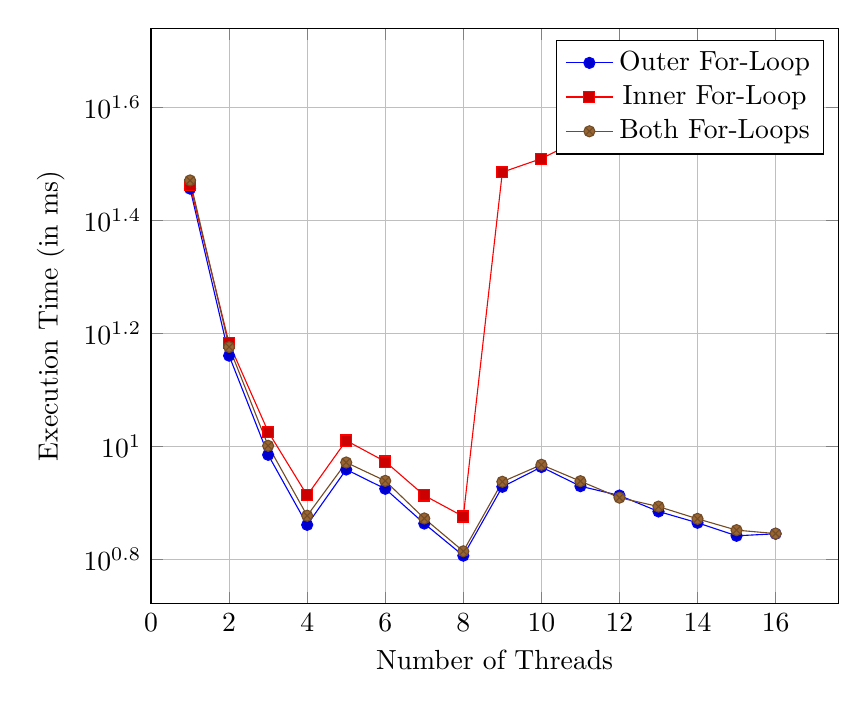
\begin{tikzpicture}
            \begin{axis}[
                title={},
                width=0.85\textwidth,
                xlabel={Number of Threads},
                ylabel={Execution Time (in ms)},
                xmin=0,
                ymin=0,
                ymode=log,
                grid=major
            ]
                \addplot coordinates {
                    (1,28.5583)(2,14.4724)(3,9.66625)(4,7.2702)(5,9.1055)(6,8.4178)(7,7.30745)(8,6.41185)(9,8.48695)(10,9.19905)(11,8.508)(12,8.1918)(13,7.677)(14,7.33135)(15,6.95245)(16,7.0099)
                };
                \addlegendentry{Outer For-Loop}

                \addplot coordinates {
                    (1,28.9709)(2,15.213)(3,10.6239)(4,8.1958)(5,10.2444)(6,9.4047)(7,8.1935)(8,7.52165)(9,30.54)(10,32.2743)(11,34.9379)(12,35.3693)(13,37.9348)(14,39.7072)(15,41.118)(16,45.1394)
                };
                \addlegendentry{Inner For-Loop}

                \addplot coordinates {
                    (1,29.5323)(2,14.9916)(3,10.0283)(4,7.545)(5,9.3703)(6,8.69475)(7,7.4621)(8,6.5289)(9,8.66325)(10,9.2846)(11,8.6837)(12,8.11935)(13,7.8319)(14,7.4501)(15,7.115)(16,7.01605)
                };
                \addlegendentry{Both For-Loops}
            \end{axis}
        \end{tikzpicture}
    \caption{Emboss Performance Tests}
    \end{figure}
\end{center}

\section{Results}

\begin{figure}[H]
    \centering

    \includegraphics[width=0.25\textwidth]{images/dice.png}
    \includegraphics[width=0.25\textwidth]{images/own-emboss.png}
    
    \caption{Results of self-implemented Emboss-Algorithm}
    \label{fig:emboss}
\end{figure}

\section{Implementation}

\begin{listing}[H]
    \begin{minted}{cpp}
cv::Mat applyEmbossOuter(cv::Mat srcImage, int numThreads = omp_get_num_procs()) {
    cv::Mat destImage(srcImage.rows, srcImage.cols, CV_8UC1);
    omp_set_num_threads(numThreads);

    #pragma omp parallel for default(none) shared(srcImage, destImage)
    for (int row = 0; row < srcImage.rows; row++) {
        for (int col = 0; col < srcImage.cols; col++) {
            int diffR, diffG, diffB, diff, gray;
            auto srcPixel = srcImage.at<cv::Vec3b>(row, col);

            if (row == 0 || col == 0) {
                diffR = srcPixel[2];
                diffG = srcPixel[1];
                diffB = srcPixel[0];
            } else {
                auto upperLeftPixel = srcImage.at<cv::Vec3b>(row - 1, col - 1);
                diffR = std::abs(srcPixel[2] - upperLeftPixel[2]);
                diffG = std::abs(srcPixel[1] - upperLeftPixel[1]);
                diffB = std::abs(srcPixel[0] - upperLeftPixel[0]);
            }

            diff = std::max(diffR, std::max(diffG, diffB));

            gray = 128 + diff;
            gray = gray > 255 ? 255 : gray;
            gray = gray < 0 ? 0 : gray;

            destImage.at<uchar>(row, col) = gray;
        }
    }

    return destImage;
}
    \end{minted}
    \captionof{lstlisting}{Emboss with parallelization of the outer For-Loop}
    \label{listing:emboss}
\end{listing}

\section{Comparison with OpenCV}

OpenCV doesn't provide an implementation on the Emboss-Algorithm.
    % \chapter{Conclusion}

\noindent
As shown in the tests above, OpenCV always performs better than the self-implemented OpenMP versions. Applying grayscale conversion is faster than converting to HSV. Emboss is the slowest of them all. \\

\noindent
All algorithms show similar performance curves. The best configuration was always 8 threads with parallelization on the outer For-Loop. The only exception made the grayscale algorithm, which performed best on 8 threads on both for Loops. The reason for that is not clear. It could be possible that grayscale uses less memory and therefore has less memory management in combination with multiple threads. Another reason could be that the CPU of the test device was throttling for a short period of time during the runtime of the test.\\

\noindent
Finally there is enough evidence that using more than 8 threads for simple algorithm like the ones presented in this documentation, doesn't yield better results on transforming images of small sizes on normal laptop like the XPS 15.


    \begin{spacing}{1.0}
        \phantomsection
        \addcontentsline{toc}{chapter}{\listfigurename}
        \listoffigures        
    \end{spacing} 

    \begin{spacing}{1.0}
        \phantomsection
        \addcontentsline{toc}{chapter}{\lstlistlistingname}
        \lstlistoflistings        
    \end{spacing}
\end{document}